\chapter{Генеративные модели}

Лектор: Алексей Сергеевич Забашта

\section{Задача генерации новых объектов}

Задачу генерации новых объектов принято относить к задаче обучения без учителя, так как нет никакого правильного варианта того, как именно генерируемые данных должны выглядеть.\newline:
При генерации стоит две задачи, между которыми необходимо искать баланс:
\begin{itemize}
    \item Мы хотим создать объект который правдоподобен в отношении некоторой скрытой структуры объектов (то есть похож на существующие объекты);
    \item Объект должен быть именно новым, а не дублем уже существующего объекта.
\end{itemize}

По заданной выборке требуется генерировать новые образцы из того же распределения. Например, на вход подается набор изображений и на выходе должен быть другой набор похожих на исходные изображений.

\begin{remark}
    Чтобы измерять сходство распределений можно использовать \textbf{дивергенцию Кульбака-Лейблера}, о которой речь шла на прошлой лекции.
\end{remark}

\begin{remark}
    Важно не забывать, что дивергенция Кульбака-Лейблера несимметрична, а значит, не является расстоянием.
\end{remark}

\begin{figure}
    \centering
    \includesvg[width=0.8\textwidth]{\detokenize{./images/taxonomy-of-generative-models.svg}}
    \caption{Таксономия генеративных моделей}
\end{figure}


\section{PixelCNN и PixelRNN}

\begin{remark}
    Такие методы еще называются \textit{авторегрессионными}.
\end{remark}

\begin{definition}
    \textbf{PixelRNN} --- это такая архитектура, которая выполняет генерацию изображения, начиная с левого верхнего угла. Зависимость от предыдущих пикселей моделируется с помощью RNN (LSTM или biLSTM, чтобы учитывать не только пиксель слева, но и пиксель сверху).
\end{definition}

\begin{definition}
    \textbf{PixelCNN} --- архитектура, аналогичная PixelRNN, также генерирующая изображения, начиная с левого верхнего угла. Таким образом, свертка по уже сгенерированным пикселям генерирует новые. Её преимущество состоит в том, что она обучается быстрее, чем PixelRNN.
\end{definition}

Обе эти архитектуры обладают следующими преимуществами:
\begin{itemize}
    \item Они могут явно вычислить правдоподобие $p(x)$;
    \item Явное правдоподобие обучающих данных дает хорошую метрику оценки;
    \item Дают хорошие образцы.
\end{itemize}

Основной их недостаток состоит в том, что они выполняют генерацию последовательно, а это медленно.

\begin{remark}
    На сегодняшний день эти методы считаются устаревшими.
\end{remark}

\section{Вариационные автокодировщики}

\begin{definition}
    \textbf{Вариационный автокодировщик} (\textit{Variational Autoencoder}, \textit{VAE}) — автокодировщик (генеративная модель, которая учится отображать объекты в заданное скрытое пространство и обратно), основанный на вариационном выводе.
\end{definition}

При использовании обычного автокодировщика для генерации новых объектов (желательно из того распределения, что и исходный набор данных) возникает следующая проблема. Неизвестны параметры распределения скрытого пространства, которые требуется установить, чтобы картинка, после применения декодера, стала похожа на картинки из исходного набора данных, но при этом не совпадала ни с одной из них. Обыкновенный автокодировщик не может ничего утверждать про распределение скрытого вектора и даже про его область определения (например, она может быть дискретной).\newline
Вариационный автокодировщик, в свою очередь, предоставляет возможность определить распределение скрытого вектора за счет наложения ограничений на него. В частности, благодаря регуляризации можно заставить сеть генерировать скрытые вектор только из стандартного нормального распределения $N(0, 1)$.\newline
В таком варианте у нас появляется возможность давать декодеру на вход вектор из $N(0, 1)$ и получать на выходе сгенерированный объект, похожий на объекты из исходного набора данных.

\begin{figure}[h]
    \centering
    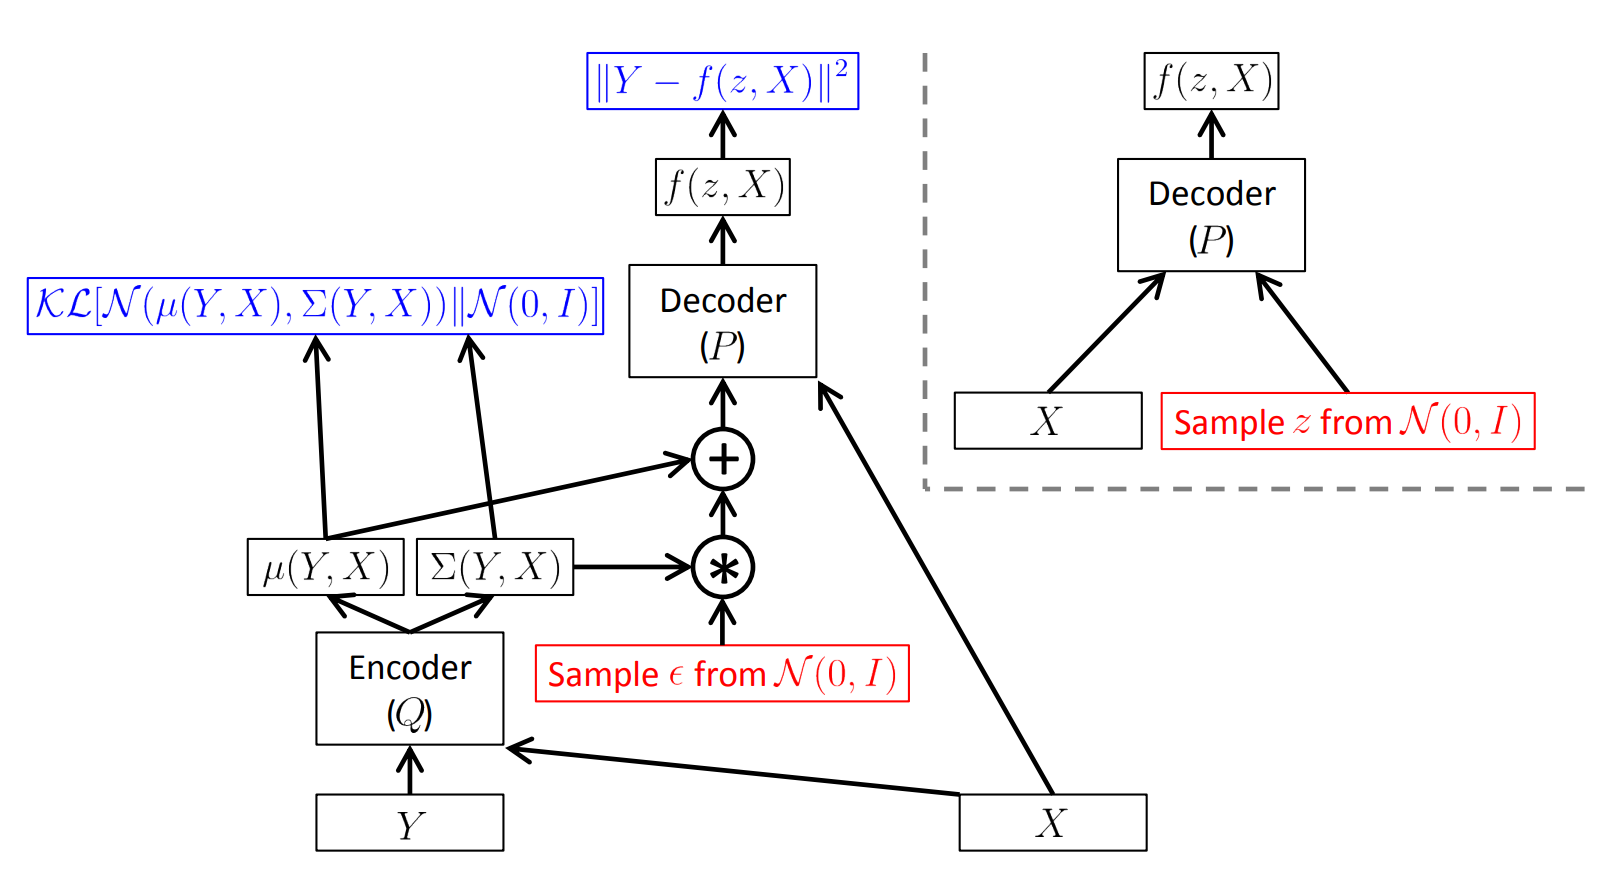
\includegraphics[width=0.9\textwidth]{images/vae.png}
    \caption{Архитектура вариационного автокодировщика}
\end{figure}

\textbf{преимущества вариационного автокодировщика}:
\begin{enumerate}
    \item Принципиальный подход к генеративным моделям;
    \item Позволяет сделать вывод $q(z|x)$, может быть полезным представлением функции для других задач.
\end{enumerate}

\textbf{Недостатки}:
\begin{enumerate}
    \item Максимизация нижней границы вероятности --- не такая хорошая оценка, как PixelRNN или PixelCNN.
    \item Образцы более размытые и более низкого качества по сравнению с современными (GAN).
\end{enumerate}

\section{Генеративно-состязательные модели}

\begin{figure}[h]
    \centering
    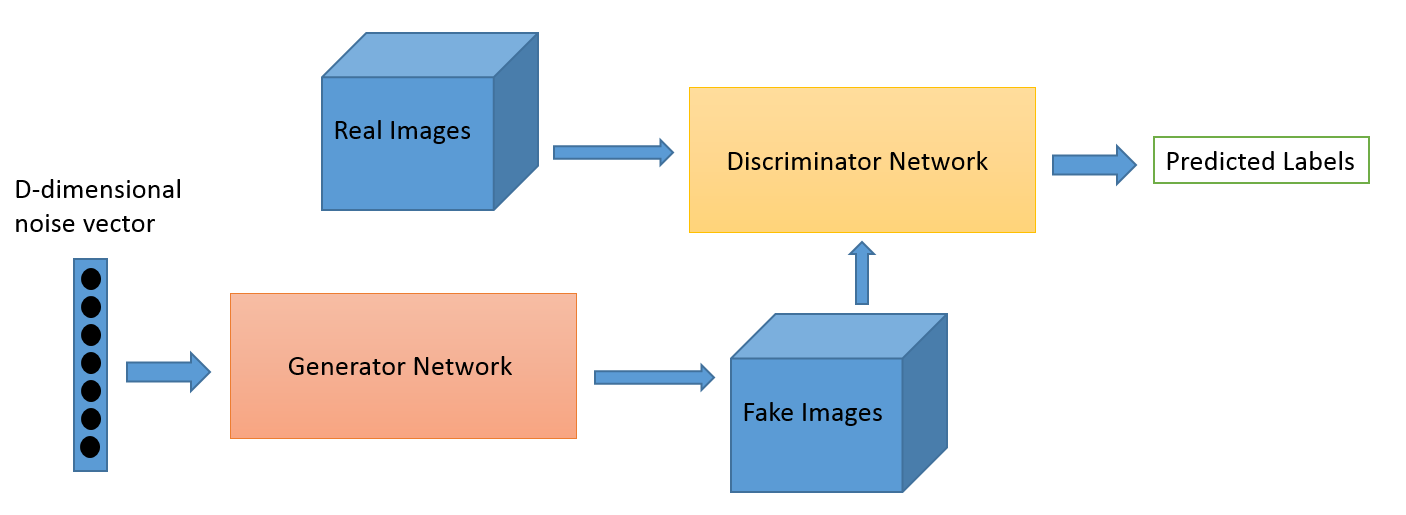
\includegraphics[width=\textwidth]{images/gan.png}
    \caption{Простая блок-схема GAN}
\end{figure}

\begin{definition}
    \textbf{Порождающие состязательные сети} (\textit{Generative Adversarial Nets}, \textit{GAN}) — алгоритм машинного обучения, входящий в семейство порождающих моделей и построенный на комбинации из двух нейронных сетей:
    \begin{enumerate}
        \item \textbf{Генератора} --- генеративной модели $G$, которая строит по вектору случайных шумов приближение распределения данных
        \item \textbf{Дискриминатора} --- дискриминативной модели $D$, оценивающей вероятность, что образец пришел из тренировочных данных, а не сгенерированных моделью $G$.
    \end{enumerate}
    Обучение для модели $G$ заключается в максимизации вероятности ошибки дискрминатора $D$.
\end{definition}

Минимаксная целевая функция выглядит следующим образом:
\[
    \min_{\theta_g}\max_{\theta_d}[\E_{x\sim p_{data}}\log D_{\theta_d}(x)+\E_{z\sim p(z)}\log(1-D_{\theta_d}(G_{\theta_g}(z)))],
\]
где
\begin{itemize}
    \item $G_{\theta_g}$ --- дискриминатор с параметрами $\theta_d$,
    \item $G_{\theta_d}$ --- генератор с параметрами $\theta_g$.
\end{itemize}

\begin{remark}
    Дискриминатор пытается максимизировать целевую функцию и сделать так, чтобы $D(x)$ был близок к 1 (настоящий) и $D(G(z))$ был близок к 0 (сгенерированный). Генератор старается него обмануть и добиться, чтобы $D(G(z))$ стал близок к 1.
\end{remark}

Обучение происходит поочередно:
\begin{enumerate}
    \item \textbf{Градиентный подъем} по дискриминатору:
    \[
        \max_{\theta_d}[\E_{x\sim p_{data}}\log D_{\theta_d}(x)+\E_{z\sim p(z)}\log(1-D_{\theta_d}(G_{\theta_g}(z)))];
    \]
    \item \textbf{Градиентный спуск} по генератору
    \[
        \min_{\theta_g}\E_{z\sim p(z)}\log(1-D_{\theta_d}(G_{\theta_g}(z))).
    \]
\end{enumerate}

\begin{remark}
    Вместо второго правила иногда используют градиентный подъем на генераторе:
    \[
        \max_{\theta_g}\E_{z\sim p(z)}\log(D_{\theta_d}(G_{\theta_g}(z))).
    \]
    Это позволяет быстрее двигаться в начале обучения, так как градиенты вблизи нуля у этой функции выше.
\end{remark}

\begin{figure}[h]
    \centering
    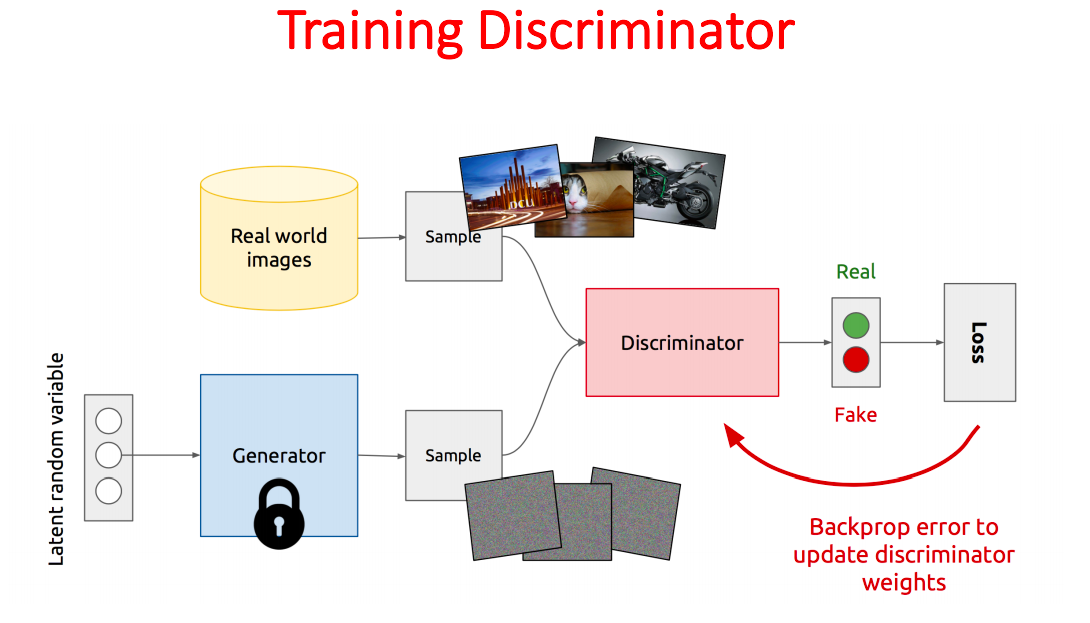
\includegraphics[width=\textwidth]{images/training-discriminator.png}
    \caption{Шаг обучения дискриминатора}
\end{figure}

\begin{figure}[h]
    \centering
    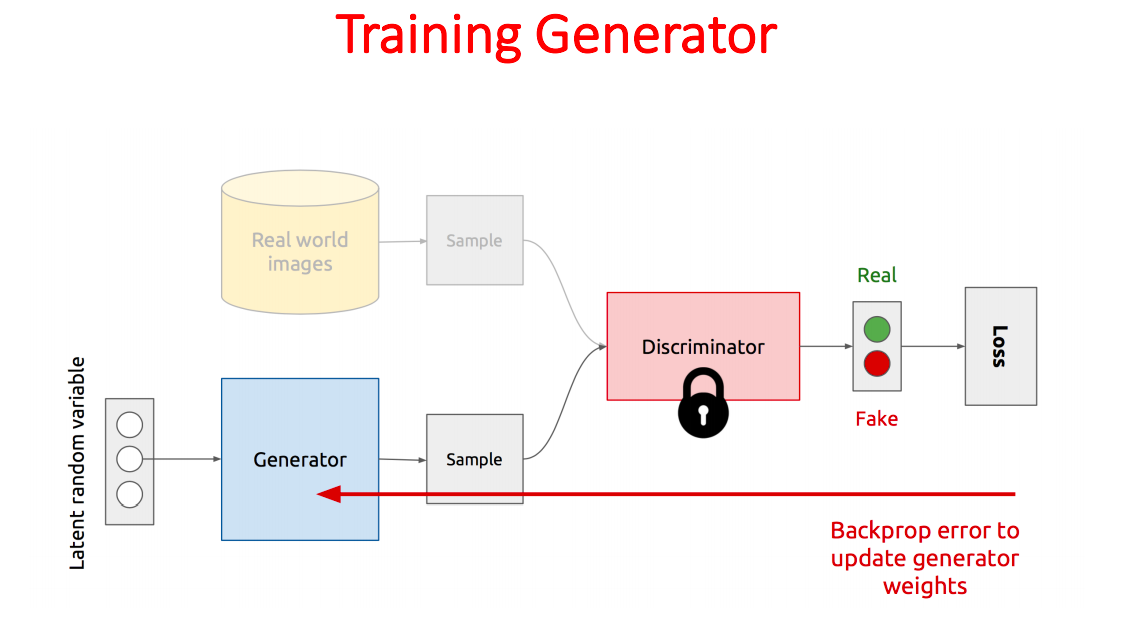
\includegraphics[width=\textwidth]{images/training-generator.png}
    \caption{Шаг обучения генератора}
\end{figure}

Недостатками GAN'ов являются:
\begin{itemize}
    \item Схлопывание мод распределения (mode collapse) --- ситуация при которой генератор всегда создает одинаковые объекты, с помощью которых у него лучше всего получается обманывать дискриминатор;
    \item Осцилляция;
    \item Нет индикатора, когда останавливаться.
\end{itemize}

\section{Интересные идеи в GAN'ах}

\begin{definition}
    \textbf{Conditional Gans} (\textit{CGANs}) --- улучшение GAN, которое позволяет добавить несколько меток, чтобы дискриминатор могу работать как классификатор по отношению к некоторым меткам. В таком случае у нас разное распределение для каждого класса, а целевая функция выглядит так:
    \[
        \min_{\theta_g}\max_{\theta_d}[\E_{x\sim p_{data}}\log D_{\theta_d}(x,y)+   \E_{z\sim p(z)}\log(1-D_{\theta_d}(G_{\theta_g}(x,y), y))]
    \]
\end{definition}

\begin{definition}
    \textbf{Задача оптимального перемещения} --- идея улучшения GAN, которая заменяет KL на расстояние Вассерштайна:
    \[
        W(p_{data},p_{gen})=\inf_{\gamma\in\prod(p_{data},p_{gen})}\E_{(x,y)\sim\gamma}[||x-y||],
    \]
    где $\prod(p_{data},p_{gen})$ --- это множество совместных распределений над $p_{data}$ и $p_{gen}$.
    \begin{remark}
        Его нельзя считать напрямую, но можно найти приблизительное решение, которое поможет бороться с mode collapse.
    \end{remark}
\end{definition}

Еще одна идея, как можно достигать хорошего качества --- усложнять генератор и дискриминатор в процессе обучения.

\begin{figure}
    \centering
    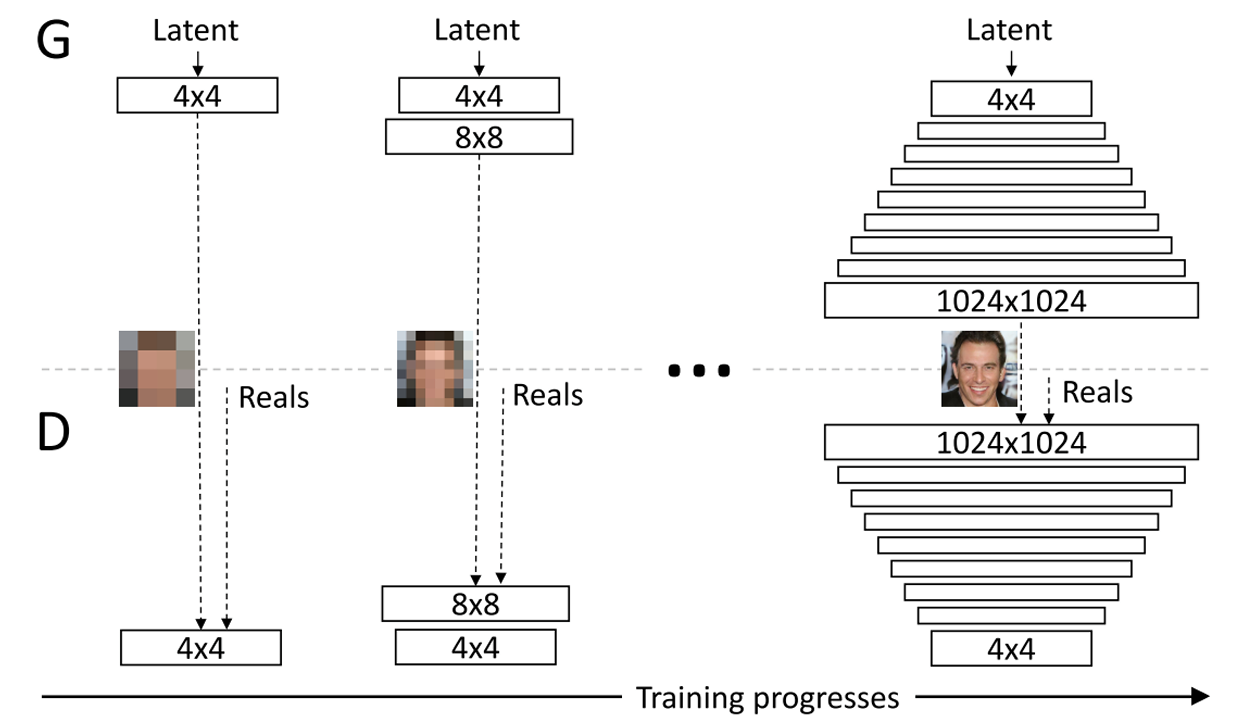
\includegraphics[width=\textwidth]{images/gan-training.png}
    \caption{Усложнение GAN в процессе обучения}
\end{figure}

\section{Диффузные модели}

\begin{remark}
    Диффузные модели сейчас наиболее популярны (пример - Midjourney).
\end{remark}

Идея метода основана на диффузии. На стадии обучения к изображению итеративно добавляется небольшой шум $q$. Модель $p$ обучается убирать этот шум. При этом можно добавить условие на то, что должно скрываться за шумом.
